\section{Basic idea of the LBM}
As previously noted, the lattice-Boltzmann method is a mesoscopic
method. This means that the modelling is neither done on a microscopic
(molecular) level nor by direct solving of the macroscopic equations
involved. The aim, in most situations with the lattice-Boltzmann
method is indeed to solve some macroscopic equation but not
direct. Instead a statistical model is used with various mesoscopic
variables that, in some limit, reproduces the macroscopic
variables. It is also possible to ensure that these variables (to some
extent) fulfil a certain macroscopic equation by using a certain
scheme.

Basically the lattice-Boltzmann method solves a discretised version of
eq. \eqref{eq:lbm:boltzmann-eq} for the distribution functions from
which the macroscopic quantities may be determined. Both the spatial
positions and the velocity space is discretised allowing the
distributions to ``sit'' only at certain positions and to stream to
neighbouring locations only in certain directions. A naive way to
visualise the evolution of $f$ is to consider the distribution
functions at the lattice nodes as pseudo particles that move along the
lattice and collide.

Usually in two dimensions the velocity space is discretised into 9
distinct velocities, more about the choice of lattice is discussed in
section \ref{sec:lbm:lattice}. In this case 9 distribution functions
are needed per node which might correspond to one or two macroscopic
variables but is indeed fewer than the number of variables needed for
a microscopic approach.

The discretised Boltzmann equation is referred to as the
lattice-Boltzmann equation (LBE) and is one of the fundamental corner
stones in the lattice-Boltzmann method, it reads:

\begin{equation}\label{eq:lbm:lbe}
f_i(\x + \cbf_i\delta_t, t + \delta_t) - f_i(\x, t) = \Omega_{ij}(\x, t)
\end{equation}
where $f_i$ denotes the distribution function for direction $\cbf_i$,
$\delta_t$ is the time step and $\Omega_ij$ is the (for now
non-specified) collision operator. An implicit sum over the second
velocity index $j$ is assumed. Various forms of collision operators
exist and will be further discussed in section \ref{sec:lbm:col}.

\subsection{Computational algorithm}
In order to solve eq. \eqref{eq:lbm:lbe} the distribution functions
must be set to some initial value. The choice of initial value is in
most cases crucial with respect to stability and accuracy of the
method. More about the initialisation will be discussed in later
sections of this chapter. 

When a proper initialisation has been performed, the time evolution of
the distribution functions is determined iteratively by the explicit
scheme in the LBE, eq. \eqref{eq:lbm:lbe}. The update in each time
step is usually divided into two computational tasks. First, the new
value that later will be propagated to a neighbouring node is computed,
i.e.

\begin{equation}
f_i^{*}(\x, t + \delta_t) = f_i(\x, t) + \Omega_{ij}(\x, t)
\end{equation}
This step will be referred to as the collision step since it is here
the ``collision'' is computed. The second step consists of propagating
the distribution functions to the neighbouring node in its
corresponding direction, i.e.
\begin{equation}
f_i(\x + \cbf_i\delta_t, t + \delta_t) = f_i^*(\x, t + \delta_t)
\end{equation}
This step will be referred to as the streaming step.

In the case of a finite domain, certain rules (boundary conditions)
must be specified at the boundaries. Typically the distribution
functions that are going to be streamed out of the domain is used to
define the unknown ones that will ``enter'' the domain. More about
boundary conditions in section \ref{sec:lbm:bound}. Thus, at each time
step, the boundary conditions must also be handled. 

This is broadly the whole computational algorithm behind the LBM, in
fig. \ref{fig:lbm:algo}, a flow scheme of the algorithm is shown.

\begin{figure}
\begin{center}
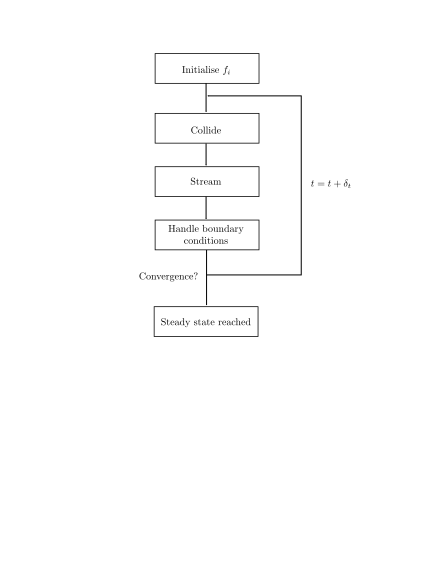
\includegraphics[width=0.5\textwidth]{fig/algorithm.pdf}
\end{center}
\caption[Flowchart of the most fundamental parts in an implementation
  of the LBM.]{Flowchart of the most fundamental parts in an implementation
  of the LBM. The convergence is usually tested for a macroscopic
  variable.}
\label{fig:lbm:algo}
\end{figure}

\nomenclature{LBE}{Lattice-Boltzmann Equation}
